\documentclass{article}
\usepackage{amsmath}
\usepackage[margin=0.5in]{geometry}
\usepackage{graphicx}
\usepackage{amsmath}
\usepackage{tikz}
\usepackage{xcolor}
\usepackage{hyperref}
\usepackage{subcaption}

\usetikzlibrary{calc, trees}

\begin{document}

\section*{Notation}

\paragraph*{Tuple Notation}

We represent a protocol distributing entanglement in a chain of $N$ nodes as a tuple
\begin{equation*}
  (PU_0, PU_1, \ldots, PU_{N-2}) \quad \text{with} \quad PU_i = \{s_i, d_i\}
\end{equation*}
representing the operations ($s$ for entanglement swapping and $d$ for distillation) to be performed on the links of the chain, after the initial entanglement generation (which is subsumed as the first operation).
\\\\
Thus, a protocol is a tuple of swaps and distillations, for example:
\begin{equation*}
    (d0, s0, d1, s2, s1)
\end{equation*}
where the first letter represents the operation to be performed, and the following number represents the segment to be distilled or, in the case of a swap, the segment to be swapped with its adjacent right one.

When two links are swapped, the new joined segment is represented by the old right segment index.
\\\\
In the example above, the protocol is composed of 2 distillations and 3 swaps, and it is performed as follows:
\begin{itemize}
    \item $d0$: distillation of segment 0,
    \item $s0$: swap of segments 0 and 1,
    \item $d1$: distillation of the joined segment of 0 and 1 (now represented as segment 1),
    \item $s2$: swap of segments 2 and 3,
    \item $s1$: final swap between the two joined segments 0-1 and 2-3.
\end{itemize}

\paragraph*{Binary Tree Notation}

Equivalently to the tuple notation, we can represent a protocol as a binary tree, where the nodes are labeled with a tuple $(i\text{-}j, k)$, where $i$ and $j$ are the extreme indices of the joined segment, and $k$ is the number of distillations performed on it, as shown in Figure \ref{fig:binary_tree_notation}.

\begin{figure}[ht!]
  \centering
  \begin{subfigure}[b]{0.45\textwidth}
    \centering
    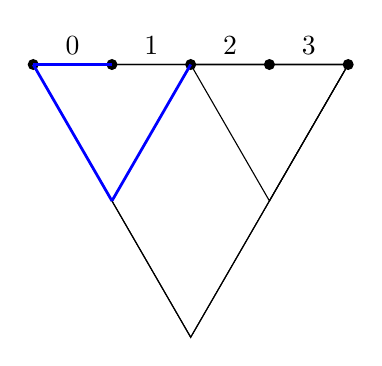
\begin{tikzpicture}
      \coordinate (A) at (0, 0);
      \coordinate (B) at (4, 0);
      \coordinate (C) at (2.0, -3.4641016151377544);

      \draw (A) -- (B) -- (C) -- cycle;

      \foreach \i in {0,1,...,3} { 
          \draw (\i, 0) -- (\i+1, 0);
      }

      \foreach \i in {0,1,...,4} { 
          \fill (\i, 0) circle (2pt);
      }

      \foreach \i in {0,1,...,3} { 
          \node[above] at ($ (\i+0.5, 0) $) {\i};
      }

      \coordinate (P0) at (0, 0);
      \coordinate (P1) at (2, 0);
      \coordinate (P2) at (1.0, -1.7320508075688772);

      \coordinate (P3) at (2, 0);
      \coordinate (P4) at (4, 0);
      \coordinate (P5) at (3.0, -1.7320508075688772);
      \draw (P3) -- (P4) -- (P5) -- cycle;

      \coordinate (P6) at (0, 0);
      \coordinate (P7) at (4, 0);
      \coordinate (P8) at (2.0, -3.4641016151377544);
      \draw (P6) -- (P7) -- (P8) -- cycle;

      \draw[blue, line width=1pt] (0,0) -- (1,0);
      \draw[blue, line width=1pt] (P0) -- (P2);
      \draw[blue, line width=1pt] (P1) -- (P2);
    \end{tikzpicture}
    \caption{}
    \label{fig:triangle_notation}
  \end{subfigure}
  \hfill
  \begin{subfigure}[b]{0.45\textwidth}
    \centering
    \begin{tikzpicture}[
      level distance=2cm,
      sibling distance=4cm,
      level 2/.style={sibling distance=2cm},
      every node/.style={inner sep=2mm}
    ]
      \node {(0-3, 0)}
          child {node {(0-1, 1)}
              child {node {(0-0, 1)}}
              child {node {(1-1, 0)}}
          }
          child {node {(2-3, 0)}
              child {node {(2-2, 0)}}
              child {node {(3-3, 0)}}
          };
    \end{tikzpicture}
    \caption{}
    \label{fig:binary_tree_notation}
  \end{subfigure}
  \label{fig:notation}
  \caption{Visual representation of the protocol $(d0, s0, d1, s2, s1)$. (\subref{fig:triangle_notation}) The triangles represent entanglement swapping operations between adjacent segments, while the blue lines represent distillation of those segments. (\subref{fig:binary_tree_notation}) A protocol can be represented as a binary tree, where the nodes are labeled with a tuple $(i\text{-}j, k)$, where $i$ and $j$ are the extreme indices of the joined segment, and $k$ is the number of distillations performed on it.}
\end{figure}
 
Considering a protocol with $N$ nodes and $S=N-1$ segments, restrictions implied by this notation are:
\begin{enumerate}
  \item a protocol must perform exactly $S$ entanglement swapping operations,
  \item $d\{i\}$ is allowed only if $s\{i\}$ has not been performed yet, otherwise the protocol is invalid.
\end{enumerate}

For example, $(d0, s0, \textcolor{red}{d0}, s2, s1)$ is not valid, as the joined segment 0-1 is represented by $1$ after entanglement swapping has been performed to join the two segments, and so $\textcolor{red}{d0}$ does not have any meaning.

\clearpage
\section*{Heterogeneous Protocols}

We also model protocols with different hardware parameter values for the freshly-generated entanglement pairs.
\\\\
For example, a 4 nodes chain
\begin{equation*}
  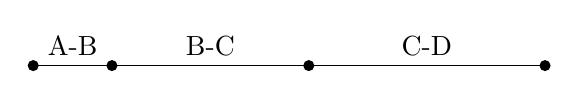
\begin{tikzpicture}
    \coordinate (A) at (0, 0);
    \coordinate (B) at (1, 0);
    \coordinate (C) at (3.5, 0);
    \coordinate (D) at (6.5, 0);
  
    \draw (A) -- (B) node[midway, above] {A-B} -- (C) node[midway, above] {B-C} -- (D) node[midway, above] {C-D};
  
    \fill (A) circle (2pt);
    \fill (B) circle (2pt);
    \fill (C) circle (2pt);
    \fill (D) circle (2pt);
  \end{tikzpicture}
\end{equation*}
can have different lengths for the segments, for example 20 km, 50 km, and 60 km, for segments A-B, B-C, and C-D, respectively, and each link can have different hardware regimes, for example:
\begin{itemize}
  \item $p_{gen} = 2.6 \cdot 10^{-3}$, $w_0 = 0.9577$ for A-B,
  \item $p_{gen} = 9.2 \cdot 10^{-4}$, $w_0 = 0.9524$ for B-C,
  \item $p_{gen} = 9.1 \cdot 10^{-4}$, $w_0 = 0.9523$ for C-D.
\end{itemize}

We can consider a time of coherence $t_{coh}^S$ for the chain given in seconds, and compute the time of coherence for each freshly generated link in time units of the simulation as:
\begin{equation*}
  t_{coh}^U = t_{coh}^S \cdot \frac{c}{L_i} \quad \text{for each segment $i$ of length $L_i$} .
\end{equation*}

Then, when performing entanglement swapping between two segments, the joint time of coherence of the memories of the two input links is given by
\begin{equation*}
  t_{\text{coh}_{i-j}} = \min(t_{\text{coh}_i}, t_{\text{coh}_j}) 
\end{equation*}
which is the minimum time of coherence of the two input links.
\\\\
For example, we can consider a coherence time of $t_{coh}^S = 20s$ for the chain, and compute the coherence times for the links as:
\begin{align*}
  t_{coh}^U &= 20s \cdot \frac{c}{20km} = 3.03 \cdot 10^{5} \quad \quad \text{for segment A-B}, \\
  t_{coh}^U &= 20s \cdot \frac{c}{50km} = 1.19 \cdot 10^{5} \quad \quad \text{for segment B-C}, \\
  t_{coh}^U &= 20s \cdot \frac{c}{60km} = 9.93 \cdot 10^{4} \quad \quad \text{for segment C-D}.
\end{align*}

When performing entanglement swapping between segments A-B and B-C, the joint coherence time will be the most restrictive one, i.e. the one of segment B-C.

\section*{Size of the Protocol Space}

The size of the protocol space is given by the number of all possible sequences of operations leading to entanglement distribution of the end-to-end link, considering the restrictions imposed by the notation.
\\\\
The number of valid possible sequences of entanglement swapping operations is given by the number of all the possible binary trees with $N$ leaves, which is given by the number of Catalan numbers of $(N-2)$. As a matter of fact, the nodes in the chain are the leaves of the binary tree, and the tree structure represents the order of the operations to be performed.
Thus, we consider all the possible binary trees with $v = 2(N-1) - 1 = 2S - 1$ vertices.
\\\\
For each valid sequence of SWAPs, we consider all the possible ways of distilling any link at any level of the chain: for each segment, we consider all the possible rounds of distillation $k$ performed on it, from 0 to a maximum $\beta$. 
This means considering, for each binary tree with $v = 2S - 1$ vertices, all the possible values of $k \in [0, \beta]$ for each vertex labeled with $(i\text{-}j, k)$.
\\\\
Thus, considering $N$ nodes, $S$ segments, and a maximum of $\beta$ rounds of distillation per segment, the size of the protocol space is given by:
\begin{equation}
    |P| = C(N-2) \cdot (\beta+1)^v
\end{equation}
where
\begin{equation}
  C(n) = \frac{1}{n+1} \binom{2n}{n}
\end{equation}
is the $n$-th Catalan number.

\clearpage
\section*{Encoding for Bayesian optimization}

We encode a protocol by starting from two real values $\gamma$ and $\zeta$:
\begin{itemize}
    \item \(\gamma\) represents the symmetricity of the protocol,
    \item \(\zeta\): represents the centering of the rounds of distillation,
\end{itemize}
they are both arbitrary real values between $0$ and $1$.
\\\\
Considering a protocol with $N=2^n+1$ for an integer $n$, the most symmetric protocol (yielded by \(\gamma=1\)), corresponds to the protocol which can be run by Boxi Li machinery.
For example, for $N=5$, the most symmetric protocol $(s0, s2, s1)$ corresponds to the protocol $(0,0)$.
All the non-symmetric protocols considered cannot be represented in the Boxi Li machinery.
\\\\
The encoding returns protocol, i.e. a tuple which represents the sequence of operations to be performed to distribute entanglement in the chain. The protocol is generated as follows.
\\\\
The set of all possible sequences of swaps $P_{swap}$ is generated. 
They are ordered by the symmetricity of the shape of the swaps, from the least symmetric to the most symmetric. The \((\gamma \times |P_{swap}|\)) sequence is selected, so that:
\begin{itemize}
    \item if \(\gamma = 0\), the least symmetric sequence is selected,
    \item if \(\gamma = 1\), the most symmetric sequence is selected.
\end{itemize}
For the selected sequence of swaps, the space $P_{joined}$ is generated. This is the set of all possible sequences involving the sequence of entanglement swapping operations and a maximum of $\beta$ rounds of distillation for each segment.
We consider all the possible joined sequences of swaps and distillations $P_{joined}$, ordered from the lowest to the highest  number of rounds of distillations performed. 
The \((\zeta \times |P_{joined}|)\) sequence is selected, such that:
\begin{itemize}
    \item if \(\zeta = 0\), the sequence with no rounds of distillation is selected,
    \item if \(\zeta = 1\), the sequence with the maximum number of rounds of distillation is selected.
\end{itemize}

\clearpage
\section*{Validation}

\begin{table}[ht!]
  \centering
  \begin{tabular}{|c|c|c|c|}
      \hline
      \multicolumn{2}{|c|}{Bruteforce} & \multicolumn{2}{c|}{Bayesian opt.} \\
      \hline
      Time Taken & Max. SKR & Time Taken & Max. SKR \\
      \hline
      \hline
      35h & $0.78 \times 10^{-4}$ & 44m & $0.78 \times 10^{-4}$ \\
      \hline
  \end{tabular}
  \caption{Bruteforce of all the \textbf{asymmetric protocols} and corresponding Bayesian optimization, considering $N=5$ and $\beta=2$, with protocol space size of $|P| = 3.645 \cdot 10^3$. The parameter regime is $p_{gen} = 9.2 \times 10^{-4}$, $w_0 = 0.952$, $t_{coh} = 1.4 \times 10^6$, equivalent to Case C of Table \ref{tab:hardware_regimes}. Bayesian optimizations are performed with 10 initial points and a total of 100 shots.}
  \label{tab:validation_regimes}
\end{table}

For the hardware parameters $p_{gen} = 9.2 \times 10^{-4}$, $w_0 = 0.952$, $t_{coh} = 1.4 \times 10^6$, we consider the case of $N=5$ nodes and $\beta=2$ rounds of distillation and present the results of the Bayesian optimization in Figure \ref{fig:gp_validation}.
\\\\
The protocol that maximizes the secret key rate is
  ('d0', 'd0', 'd1', 'd1', 's0', 'd2', 'd2', 'd3', 'd3', 's2', 's1')
which corresponds to the maximally symmetric protocol $(1,1,0,0)$.

\begin{figure}[ht!]
  \centering
  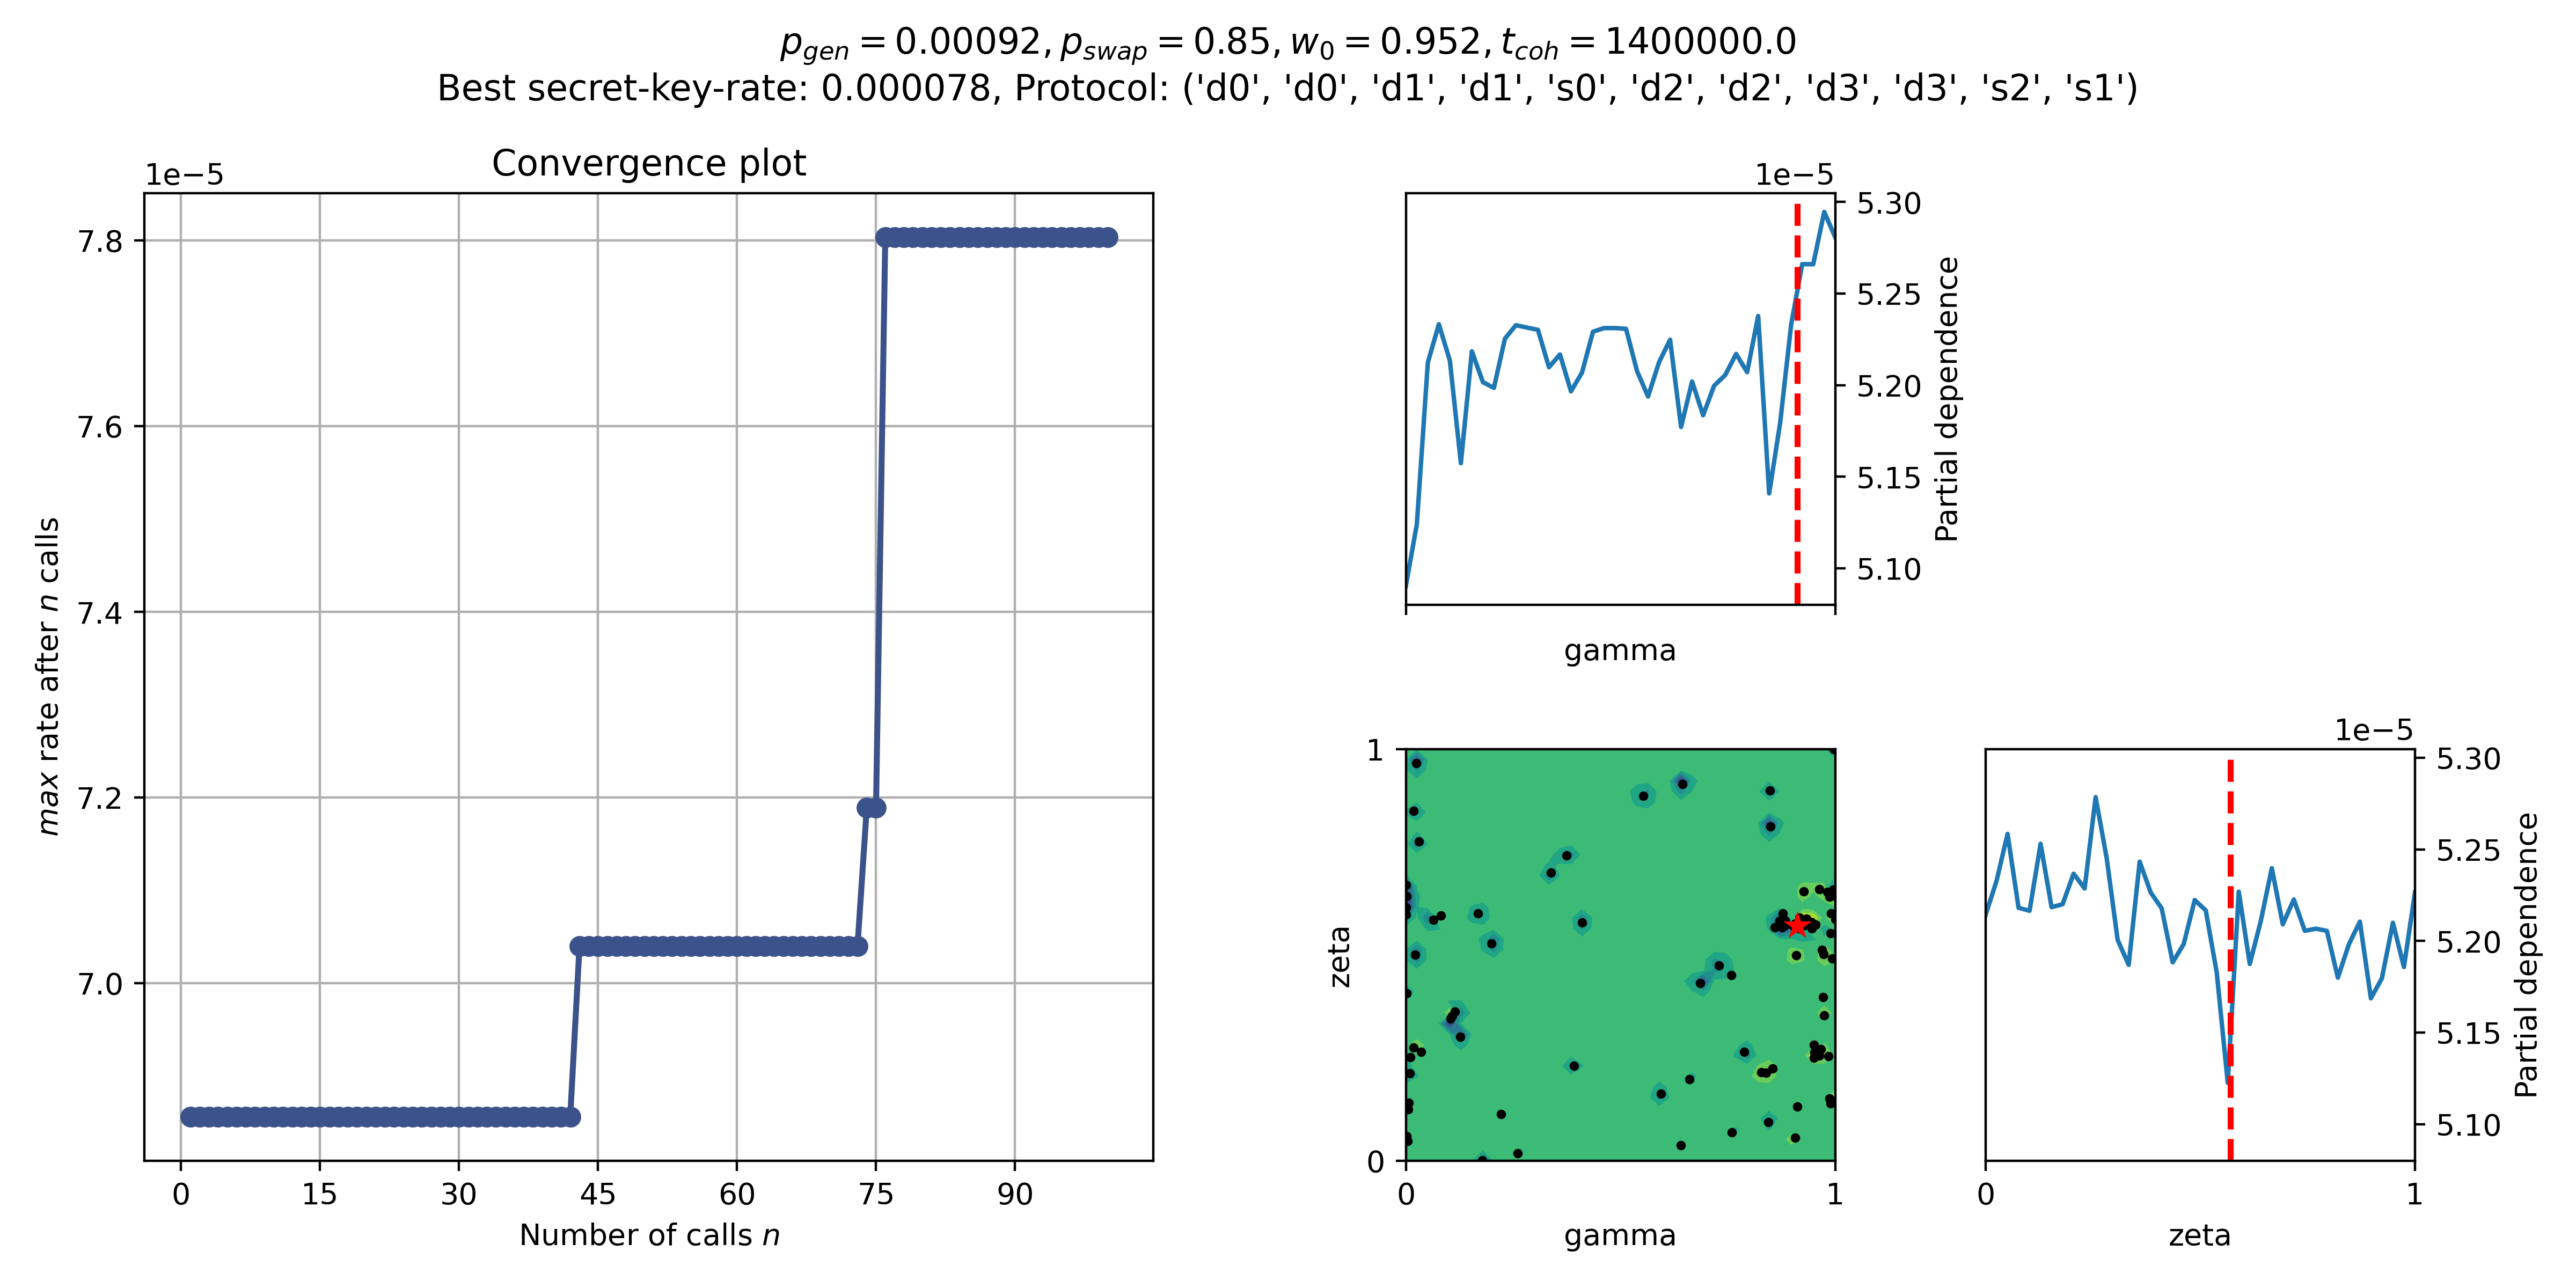
\includegraphics[width=\linewidth, trim=10 10 10 40, clip]{asymmetric/gp5,2/skopt_gp.png}
  \caption{Results of the Bayesian optimization for $N=5$ and $\beta=2$. The algorithm converges to the optimal protocol in less than 100 evaluations, while a bruteforce algorithm must evaluate all the 3645 protocols.}
  \label{fig:gp_validation}
\end{figure}

\clearpage
\section*{Results}

We present the results of the Bayesian optimization for symmetric and asymmetric protocols, for different hardware regimes and number of nodes.
\\\\
In Table \ref{tab:hardware_regimes}, we present the hardware regimes considered, with the corresponding values of $L_0$, $t_{coh}$, $w_0$, and $p_{gen}$. Values for distance, initial link quality, and generation probability are chosen from the paper of Da Silva \textit{et al.}.
\\\\
In Tables \ref{tab:symmetric_protocols} and \ref{tab:asymmetric_protocols}, we present respectively the results of the Bayesian optimization for symmetric and asymmetric protocols, for different number of nodes and rounds of distillation. For each case, we present the time taken by the bruteforce and the Bayesian optimization algorithms, the maximum secret key rate obtained by both, and the size of the protocol space.

\begin{table}[ht]
    \centering
    \begin{tabular}{|c|c|c|c|c|c|}
        \hline
        Description & $L_0$ (km) & $t_{\text{coh}}$ & $w_0$($F_0$) & $p_{gen}$ \\
        \hline
        \hline
        A: Baseline value, 2 nodes & 200  & $3.6 \times 10^5$ & 0.36 (0.52) & $9.6 \times 10^{-8}$ \\
        \hline
        B: Baseline value, 3 nodes & 100  & $7.2 \times 10^5$ & 0.867 (0.9) & $1.5 \times 10^{-5}$ \\
        \hline
        C: The Hague - Leiden, 5 nodes & 50  & $1.4 \times 10^6$ & 0.952 (0.964) & $9.2 \times 10^{-4}$ \\
        \hline
        D: Delft - The Hague, 11 nodes & 20  & $3.6 \times 10^6$ & 0.958 (0.968) & $2.6 \times 10^{-3}$ \\
        \hline
    \end{tabular}
    \caption{\textbf{Hardware Regimes} considered for the simulations. $L_0$ is the distance between the nodes of the chain, $w_0$ is the quality of a freshly-generated link, and $p_{gen}$ is the probability of successful generation of an entangled pairs at link level. $t_{coh}$ is the joint coherence time of the memories of the nodes, given in units of time of the simulation.}
    \label{tab:hardware_regimes}
\end{table}

\begin{table}[ht]
    \centering
    \begin{tabular}{|c|c|c|c|c|c|}
        \hline
        & BF time & BF Results & GP time & GP result & $|P|$ \\
        \hline
        \hline
        B & 2h 32m & 0.0 & 19min & 0.0 & 21 \\
        & & (no best) & & (no best) & \\
        \hline
        C & 17min & $0.78 \times 10^{-4}$ & 6min & $0.78 \times 10^{-4}$ & 56 \\
        & & (1,1,0,0) & & $(1,1,0,0)$ & \\
        \hline
    \end{tabular}
    \caption{\textbf{Symmetric Protocols}, involving different values for $N$, depending on the row, and up to 5 rounds of distillation. All the simulations have been run on the Deigo cluster. Bayesian optimizations are performed with 2 initial points and a total of 20 shots.}
    \label{tab:symmetric_protocols}
\end{table}

\begin{table}[ht]
    \centering
    \begin{tabular}{|c|c|c|c|c|c|}
        \hline
        & BF time & BF Results & GP time & GP result & $|P|$ \\
        \hline
        \hline
        A & 5m & 0.0 & - & - & 2 \\
        \hline
        B & 95m & 0.0 & - & - & 4 \\
        \hline
        C & 116m & $0.74 \times 10^{-4}$ & 26m & $0.74 \times 10^{-4}$ & 320 \\
        \hline
        D & - & - & 6h & $4.21 \times 10^{-5}$ & $1.27 \times 10^9$ \\
        \hline
    \end{tabular}
    \caption{\textbf{Asymmetric Protocols} results. For all the cases we allowed $\beta=1$ possible rounds of distillation for each segment. All the simulations have been run on the Deigo cluster. Bayesian optimizations are performed with 10 initial points and a total of 100 shots.}
    \label{tab:asymmetric_protocols}
\end{table}

We present Case C of Table \ref{tab:symmetric_protocols} in Figure \ref{fig:symmetric_5_nodes}. The protocol that maximizes the secret key rate is $(1,1,0,0)$, a result which is consistent with the bruteforce algorithm and with the results of the validation presented in Table \ref{tab:validation_regimes}.
\\\\
We also present Case D of Table \ref{tab:asymmetric_protocols} in Figure \ref{fig:asymmetric_11_nodes}. The protocol that maximizes the secret key rate is 
\begin{equation*}
  \text{('s0', 's2', 'd1', 'd3', 's1', 'd4', 'd5', 's4', 'd3', 'd5', 's3', 's7', 'd8', 'd9', 's8', 'd6', 'd9', 's6', 'd5', 'd9', 's5', 'd9')} . 
\end{equation*}


% TODO: update with the new results
\begin{figure}[ht!]
  \centering
  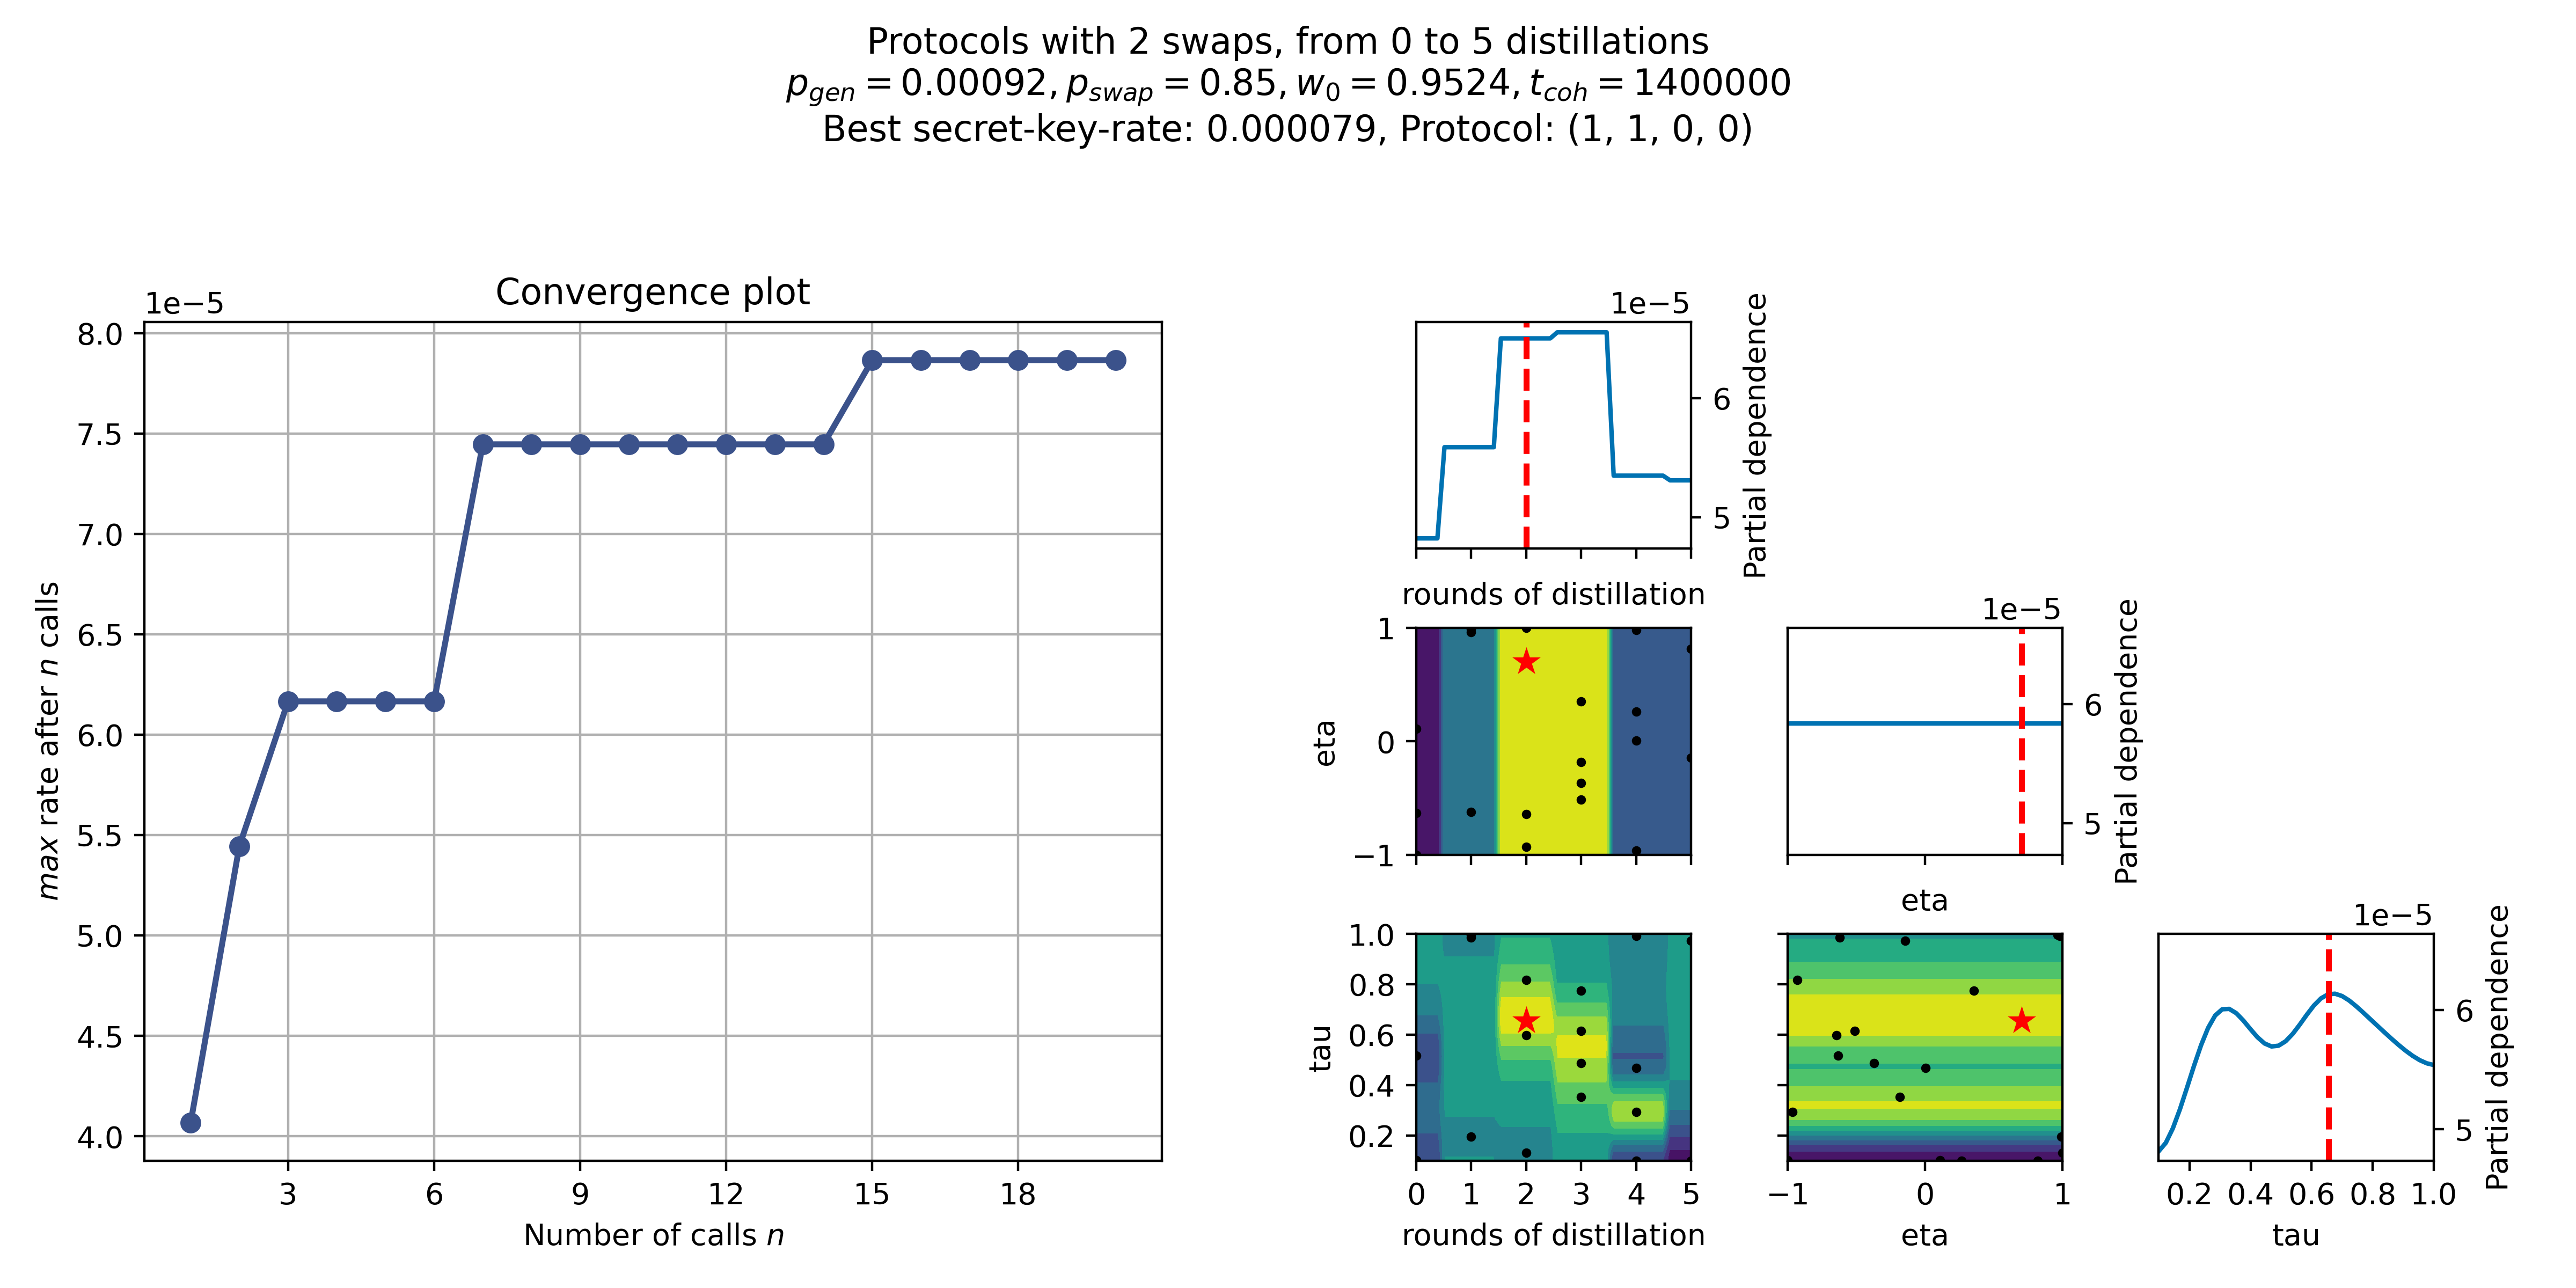
\includegraphics[width=\linewidth, trim = 10 10 10 50, clip]{symmetric/results_gp_centerspace/0.9524_2_swaps_skopt_gp.png}
  \caption{Results of the GP optimization for 5 nodes (2 symmetric swaps), and up to 5 rounds of distillation (applied to all links in the level). The algorithm converges to the optimal protocol in less than 20 evaluations, while a bruteforce algorithm must evaluate 56 protocols.}
  \label{fig:symmetric_5_nodes}
\end{figure}

\begin{figure}[ht!]
  \centering
  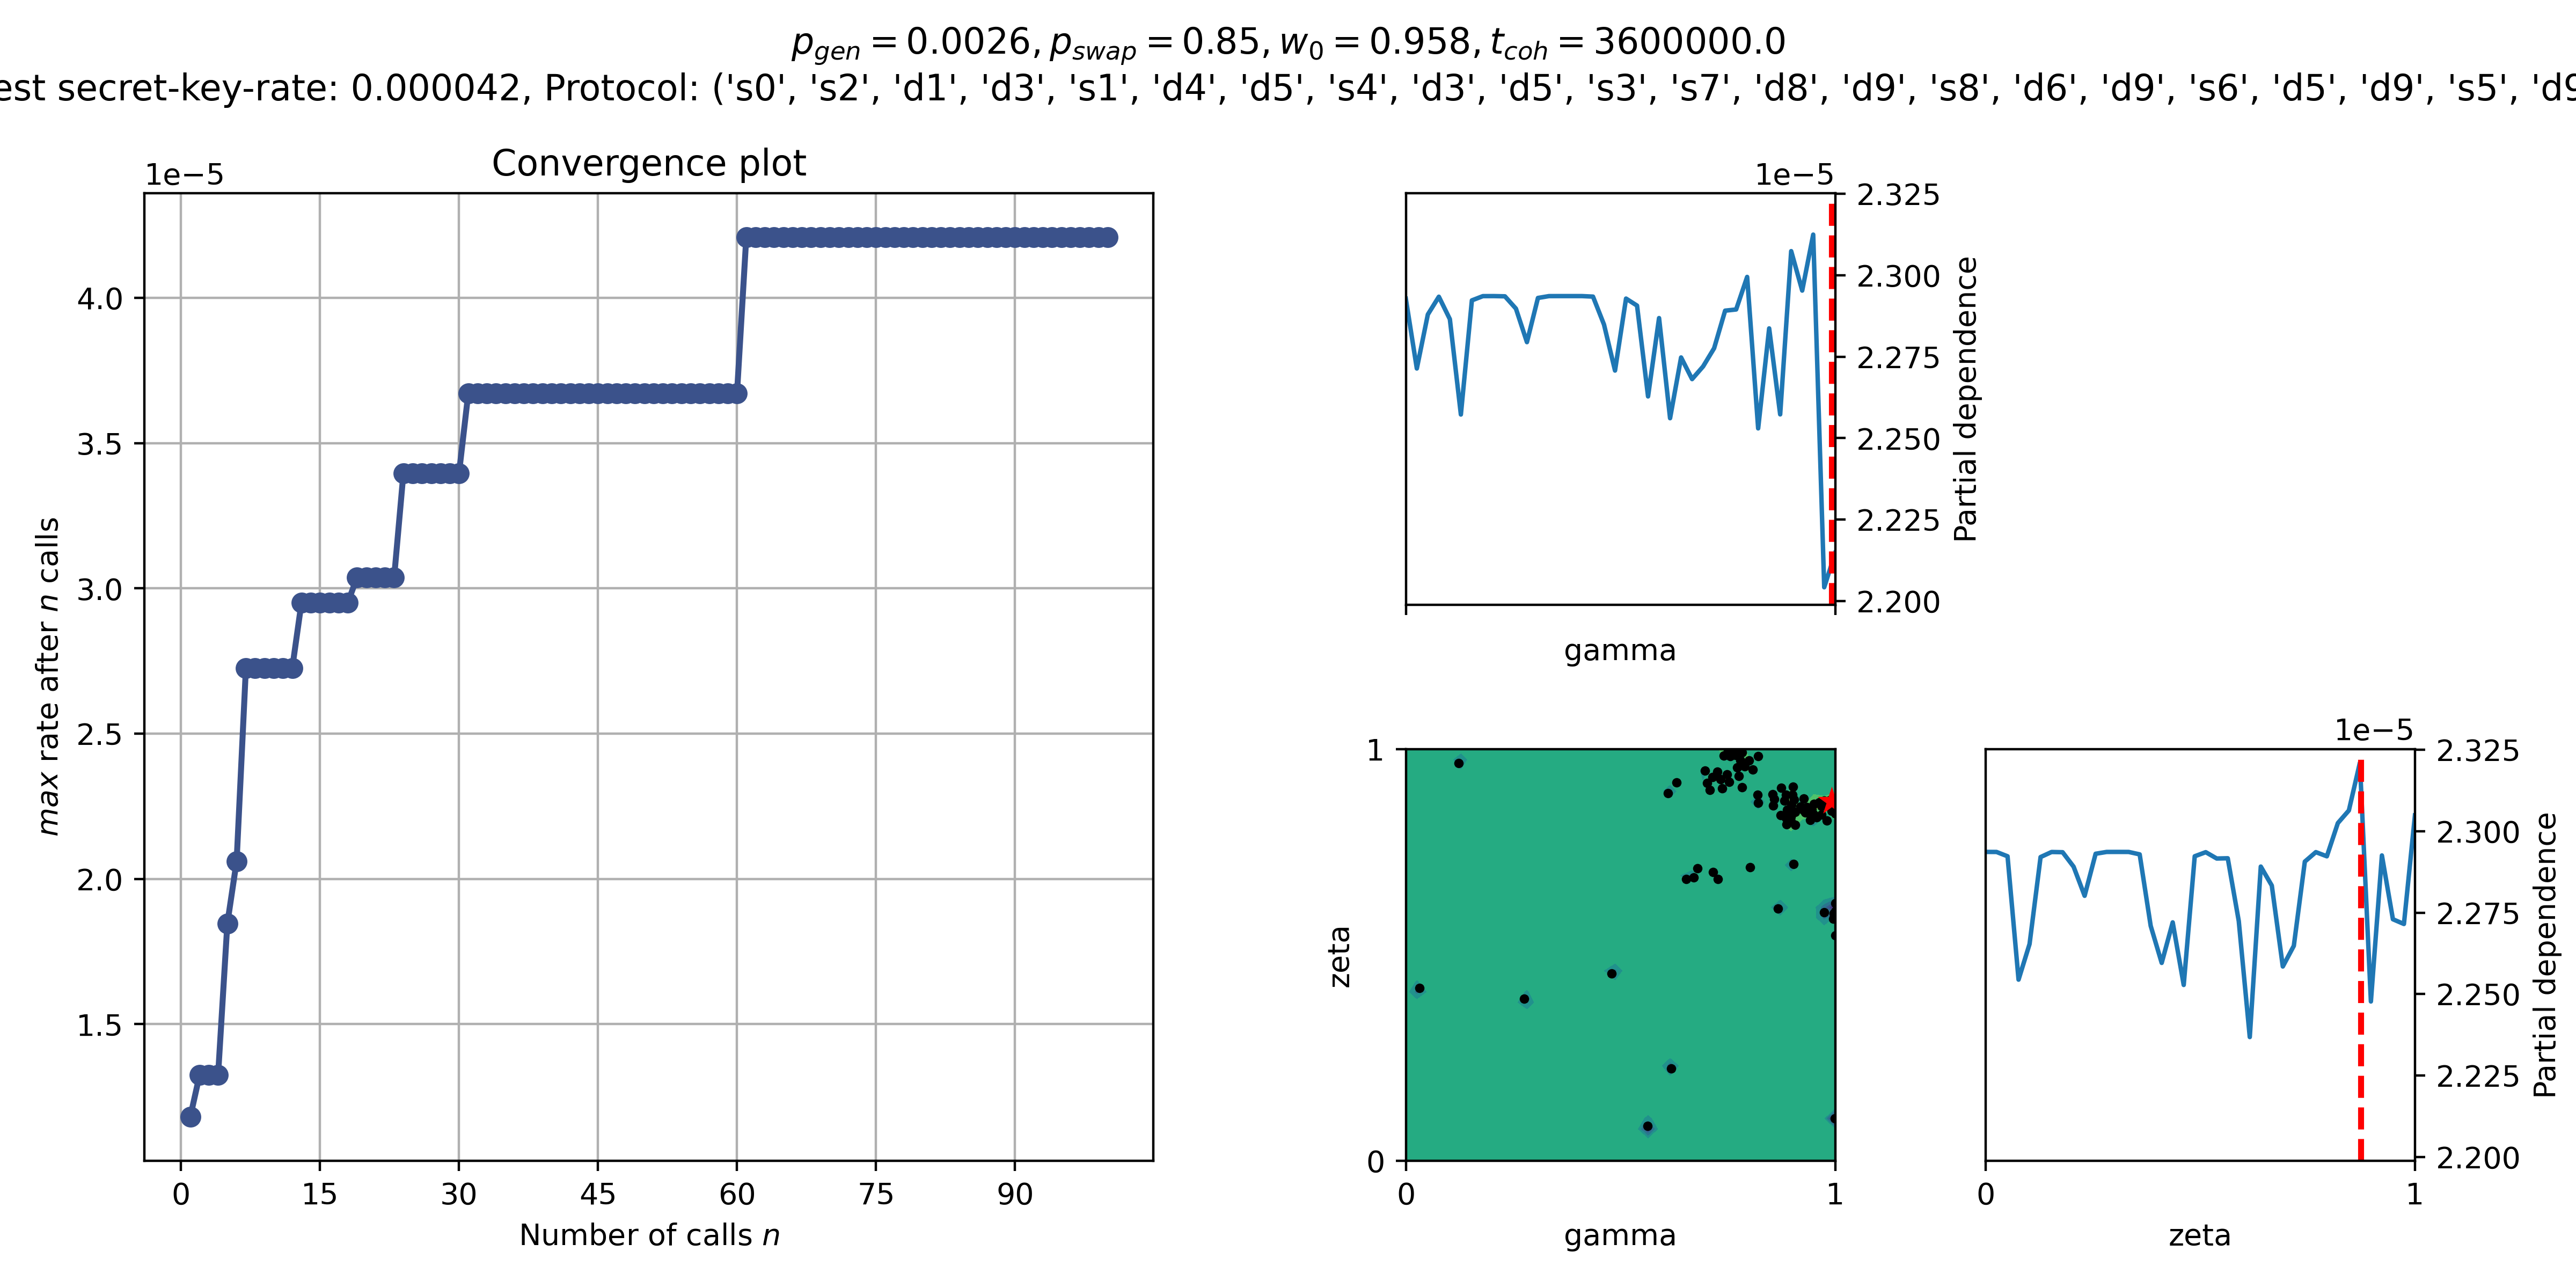
\includegraphics[width=\linewidth, trim = 10 10 10 50, clip]{asymmetric/gp11,1/skopt_gp.png}
  \caption{Results of the GP optimization for 11 nodes (asymmetric protocol), and up to 1 round of distillation for each link at any level. The algorithm converges to the maximum in less then $100$ evaluations, out of the $1.27 \times 10^9$ possible protocols.}
  \label{fig:asymmetric_11_nodes}
\end{figure}

\end{document}
